\lecture{31}{25 Mar. 10:00}{Cellular Homology}
\begin{example}
	Consider the composition of the quotient maps below $S^n \to \RP^n \to \RP^n/\RP^{n - 1} \cong S^n$. We want to compute the degree of this map.

	Note that this restricts to a homeomorphism on each component of $S^n \setminus \text{equator}$ as a map to $\RP^n \setminus \RP^{n - 1}$. Suppose we've oriented our copies of $S^n$ in such a way that the homeomorphism on the top hemisphere is orientation-preserving. The homeomorphism on the bottom hemisphere is given by taking the antipodal map and composing with the homeomorphism of the top hemisphere
	\begin{align*}
		\deg = \deg(\Id) = \deg(\text{antipodal}) = 1 + (-1)^{n + 1} = \twodef{0}{n \text{ even}}{2}{n \text{ odd}}
	\end{align*}
\end{example}

\subsection{Cellular Homology}

Suppose that $X$ is a CW complex. Then $(X^n, X^{n - 1})$ is a good pair for all $n > 1$, and $X^n/X^{n - 1}$ is a wedge of $n$-spheres, one for each $n$-cell $e^n_\alpha$. Hence:
\begin{align*}
	H_k(X^n, X^{n - 1}) \cong \twodef{0}{k \neq n}{\langle e_\alpha^n \st e_\alpha^n \text{ is an $n$-cell} \rangle }{k = n}
\end{align*}
\begin{defn}\label{defn-cellular-chain-groups}
	The cellular chain complex of $X$ has chain groups $H_n(X^n, X^{n - 1})$ with $X^{-1} = \0$.

	The boundary maps are given as:
	\begin{align*}
		d_1 : H_1(X^1, X^0)            & \to H_0(X^0)                       \\
		\langle \text{1-cells} \rangle & \to \langle \text{0-cells} \rangle
	\end{align*}
	is the usual simplicial boundary map. FOr $n > 1$, the boundayr map:
	\begin{align*}
		d_n(e_\alpha^n) = \sum_\beta d_{\alpha\beta} e_\beta^{n - 1}
	\end{align*}
	where $d_{\alpha\beta}$ is the degree of the map:
	\begin{align*}
		\xymatrix@=1.5in{
		\partial e^n_\alpha = S^{n - 1}_\alpha \ar[r]^-{\text{attaching map}} & X^{n - 1}\ar[r]^-{\text{quotient by } X^{n-1}\setminus e^{n - 1}_\beta} & S^{n-1}_\beta
		}
	\end{align*}
	In pictures, this is given as:
	\begin{center}
		%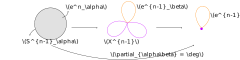
\includegraphics[scale=0.5]{cellular-boundary-map}
	\end{center}
\end{defn}

\begin{theorem}\label{thm-cellular-homology-coincides}
	The homology groups of the cellular chain complex (cellular homology groups) coincide with the singular homology groups.
\end{theorem}

\begin{corollary}[of \Cref{thm-cellular-homology-coincides}]
	We get a good bit of mileage out of this theorem:
	\begin{itemize}
		\item $H_n(X) = 0$ if $X$ has a CW-complex structure with no $n$-cells.
		\item If $X$ has a CW complex with $k$ $n$-cells, then $H_n(X)$ is generated by at most $k$ elements.
		\item If $H_n(X)$ is a group with a minimum of $k$ generators, then any CW complex structure on $X$ must have at least $k$ $n$-cells.
		\item If $X$ has a CW complex with no cells in conscecutive dimensions, then its homology is free abelian on its $n$-cells. For example $S^n, n \geq 2$ or $\CP^n$.
	\end{itemize}
\end{corollary}

\begin{example}
	$S^n$ with $n \geq 2$, using the CW coplex structure of $e^n$ attached to a single point $x_0$. The cellular chain complex is given as:
	\begin{align*}
		\xymatrix{
		0 \ar[r] & 0 \ar[r] & \langle e^n\rangle \ar[r] & 0 \ar[r] & \cdots \ar[r] & 0 \ar[r] & \langle x_0 \rangle
		}
	\end{align*}
	So then all the boundary maps are zero and we see that:
	\begin{align*}
		H_k(S^n) = \twodefo{\ZZ}{k = 0, n}{0}
	\end{align*}
\end{example}

\begin{exercise}
	Redo this calculation with other CW complex structure on $S^n$, e.g. glue 2 $n$-cells onto $S^{n - 1}$ and proceed inductively.
\end{exercise}

\begin{example}
	Let's do this with the torus
	\begin{center}
		\includegraphics[scale=0.5]{cw-complex-on-torus}
	\end{center}
	The chain complex looks like:
	\begin{align*}
		\xymatrix{
		0 \ar[r] & \langle D \rangle \ar[r]^-{\partial_2} & \langle a, b \rangle \ar[r]^-{\partial_1} & \langle x \rangle \ar[r] & 0
		}
	\end{align*}
	Note that $a \mapsto x - x = 0$ and $b \mapsto x - x = 0$ and so $\partial_1 = 0$. Now $D$ is glued along $aba^{-1}b^{-1}$, so we look at the composed up map
	\begin{center}
		\includegraphics[scale=0.5]{cellular-homology-calc-torus}
	\end{center}
	We wind forwards then backwards around $a$, so the degree is zero. The same thing happens for $b$ so:
	\begin{align*}
		\partial_2 D = 0 \cdot a + 0 \cdot b = 0
	\end{align*}
	This gives a nice \ul{principle}: If a $2$-cell $D$ is glued down via some word $w$ (this only makes sense for $2$-cells), then the coefficient to a letter $b$ in $\partial_2 D$ is the sum of the exponents of $b$ in $w$.

	Great! Now we just have that the homology groups are equal to the chain groups because the boundary maps are all zero.
\end{example}

\begin{example}
	A genus $g$ surface $\Sigma_g$ has the CW complex strucutre:
	\begin{itemize}
		\item 1 $0$-cell $x$
		\item 2g $1$-cells $a_1, b_1, a_2, b_2, \ldots$
		\item 1 $2$-cell $D$ glued along $[a_1, b_2][a_2, b_2]\cdots[a_g, b_g]$ (a product of commutators)
	\end{itemize}
	We obtain the result that:
	\begin{align*}
		\partial_1(a_i) = \partial_1(b_i) = x - x = 0
	\end{align*}
	Furthermore by the principle discussed above, we know that every $1$-cell appears once in the word, and its inverse appears once, so all the coefficients of $1$-cells in $\partial_2(D)$ are zero, so $\partial_2(D) = 0$. This means we have a chain complex:
	\begin{align*}
		\xymatrix{
		0 \ar[r] & \ZZ \ar[r]^-{0} & \ZZ^{2g} \ar[r]^-{0} & \ZZ \ar[r] & 0
		}
	\end{align*}
	And so then we have that:
	\begin{align*}
		H_k(\Sigma_g) = \threedefo{\ZZ}{k = 0, 2}{\ZZ^{2g}}{k = 1}{0}
	\end{align*}
\end{example}

\begin{example}[Torus example: $\partial_2$ in more detail]
	We're going to work through this example a bit more carefully.
	\begin{center}
		\includegraphics[scale=0.5]{more-careful-torus-cellular}
	\end{center}
	Let's zoom in on these two preimage points and use local homology to compute this:
	\begin{center}
		\includegraphics[scale=0.5]{zoom-torus-cellular-preimage}
	\end{center}
\end{example}